%!TEX root = ../template.tex
%%%%%%%%%%%%%%%%%%%%%%%%%%%%%%%%%%%%%%%%%%%%%%%%%%%%%%%%%%%%%%%%%%%%
%% annex1.tex
%% NOVA thesis document file
%%
%% Chapter with example of appendix with a short dummy text
%%%%%%%%%%%%%%%%%%%%%%%%%%%%%%%%%%%%%%%%%%%%%%%%%%%%%%%%%%%%%%%%%%%%

\typeout{NT FILE annex1.tex}

\chapter{Annex 1 Configuring R-IoT}
\label{ann:riot_opensignals}

The screenshots below overview the configuration steps required to stream data between the R-IoT device and host computer over a local WiFi network. As part of our technical preparations described in Section \ref{technical_contributions:severbit}, we developed a middleware program to simplify this process. These are specifically directed to the OpenSignals software package, though the general procedure may applied to other applications also.

\begin{center}
    % \begin{figure}[H]
      % \centering
    \includegraphics[width=0.6\linewidth]{Chapters/Figures/annex-appendix/serverBIT/riot_opensignals_5.png}
    % \caption{}
    \label{fig:riot_opensignals_5}
    % \end{figure}
    
    % \begin{figure}[H]
      % \centering
    \includegraphics[width=0.6\linewidth]{Chapters/Figures/annex-appendix/serverBIT/riot_opensignals_12.png}
    % \caption{}
    \label{fig:riot_opensignals_12}
    % \end{figure}
    
    % \begin{figure}[H]
      % \centering
    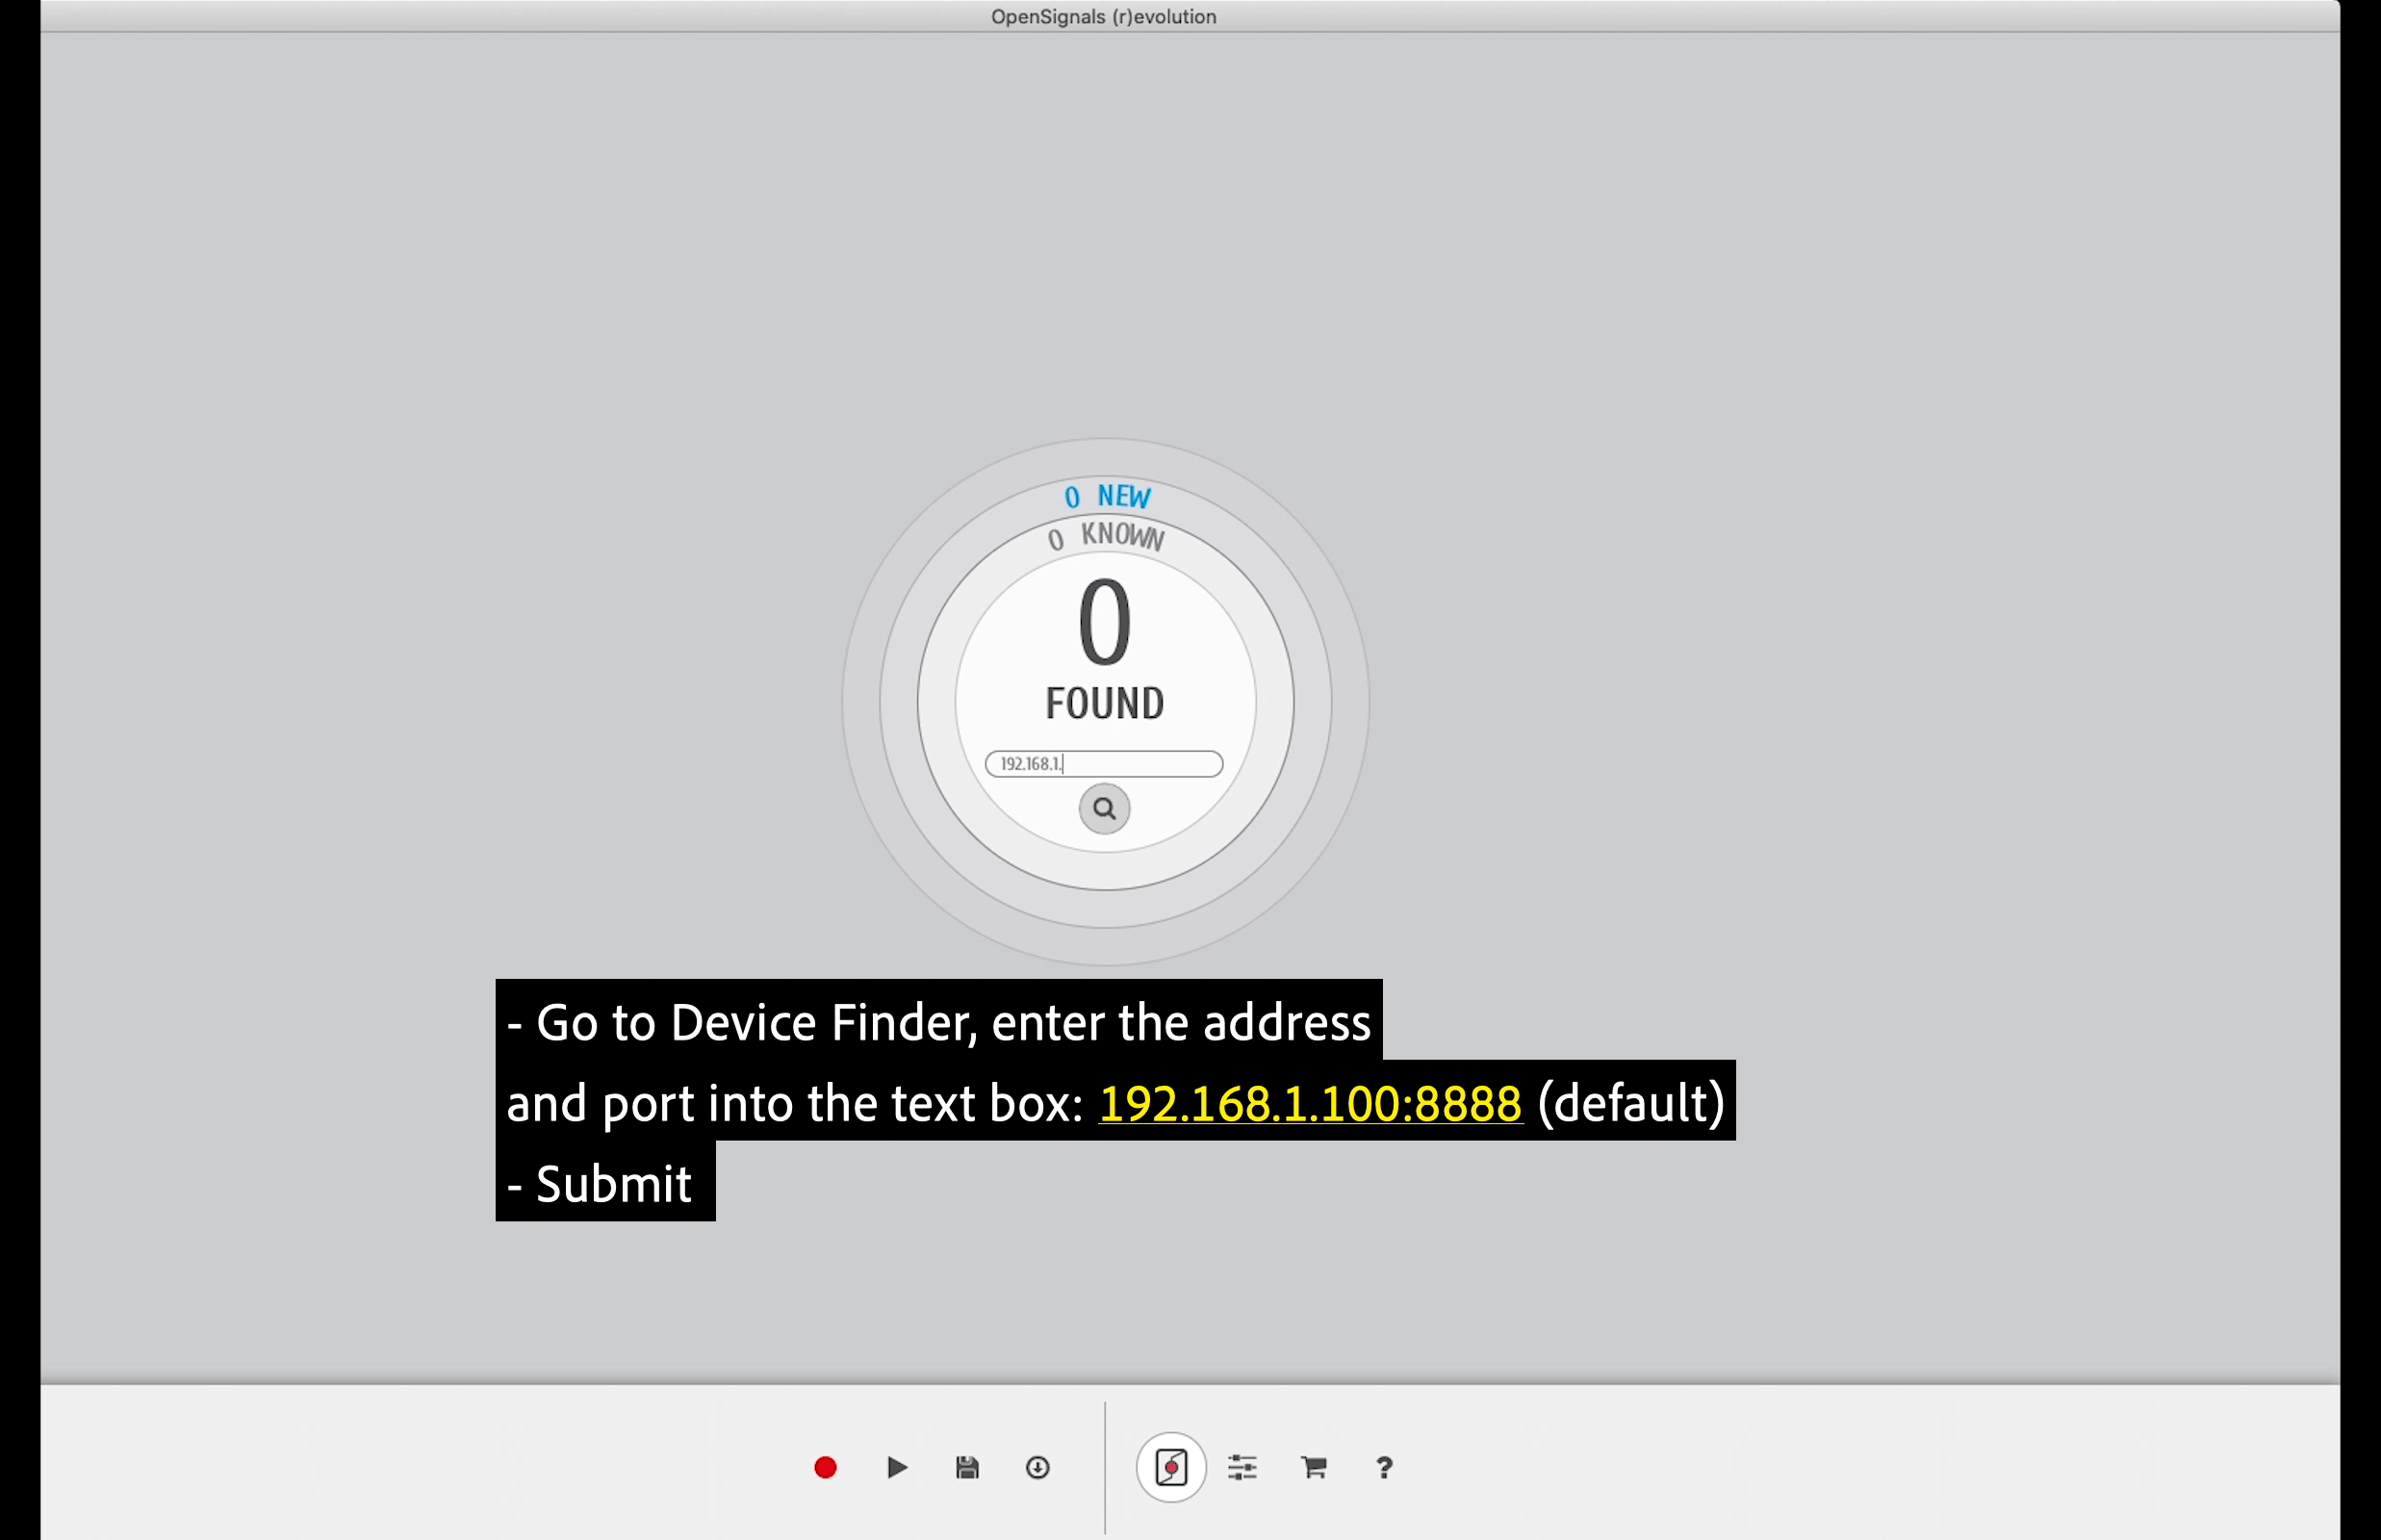
\includegraphics[width=0.6\linewidth]{Chapters/Figures/annex-appendix/serverBIT/riot_opensignals_45.png}
    % \caption{}
    \label{fig:riot_opensignals_45}
    % \end{figure}
    
    % \begin{figure}[H]
      % \centering
    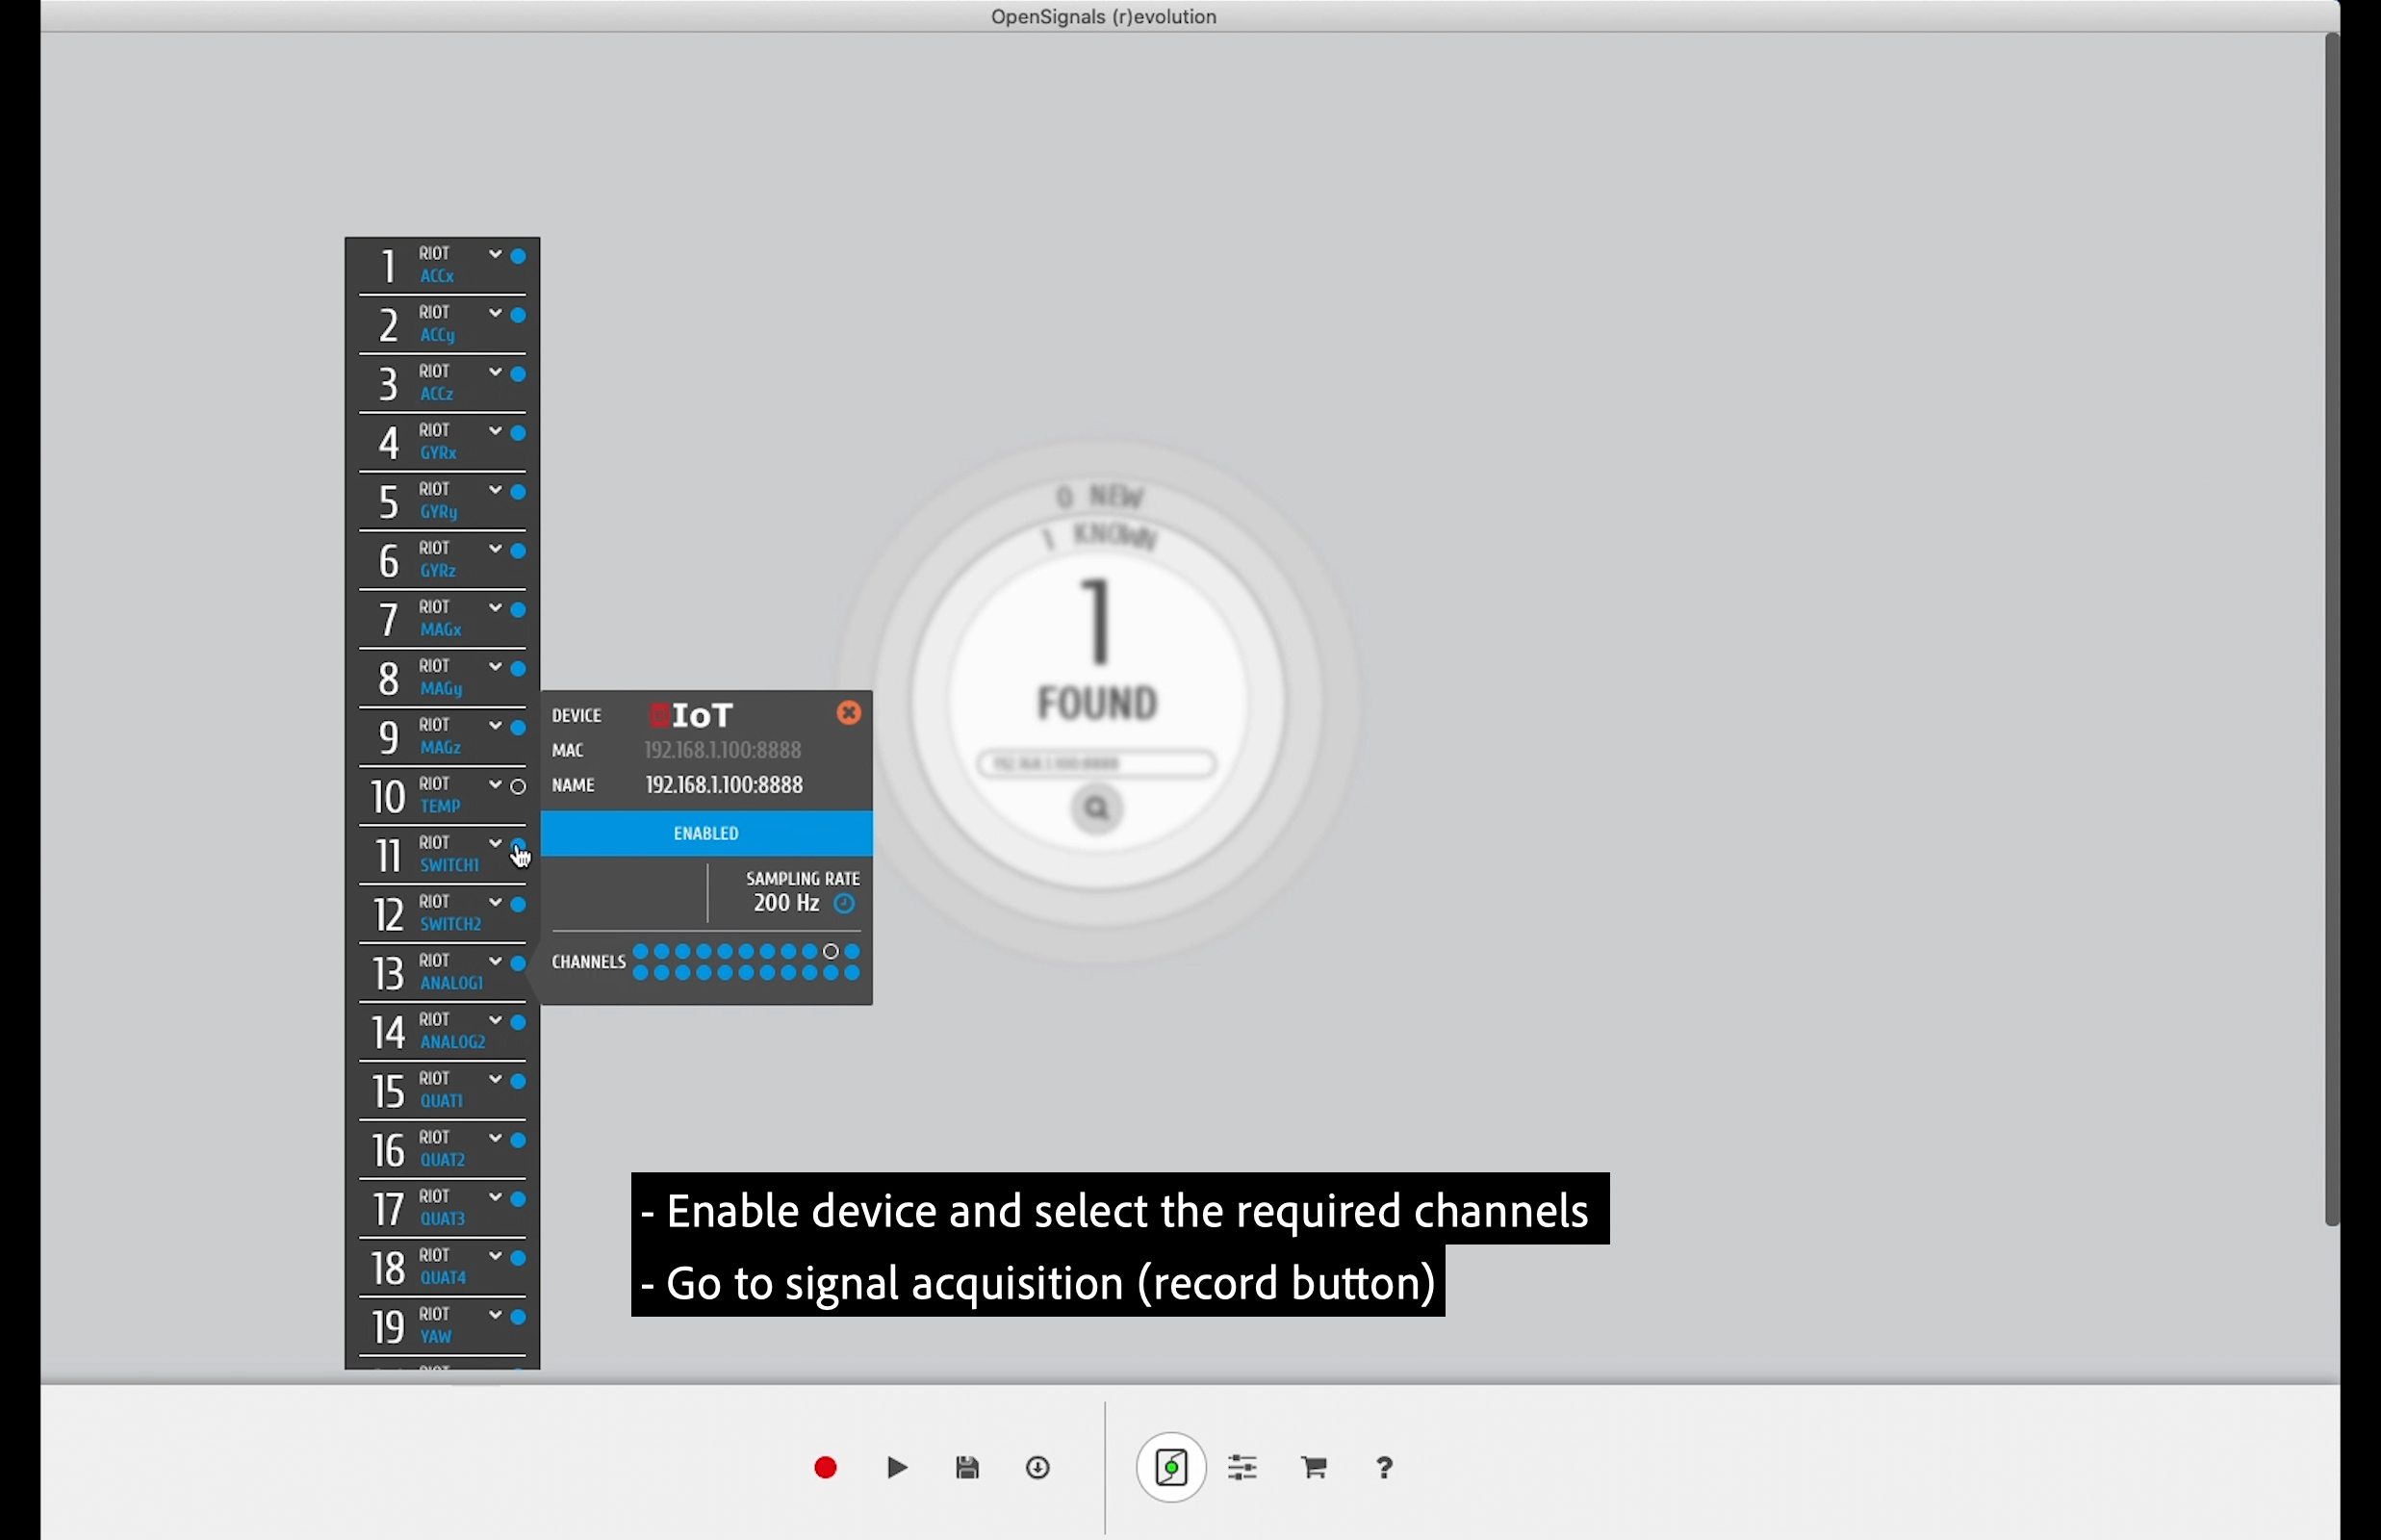
\includegraphics[width=0.6\linewidth]{Chapters/Figures/annex-appendix/serverBIT/riot_opensignals_71.png}
    % \caption{}
    \label{fig:riot_opensignals_71}
    % \end{figure}
\end{center}

\begin{enumerate}
    \item Power on the device. Connect to the local WiFi network assigned to the R-IoT Configuration
    \item Change the IP address to static/manual and alter according to the R-IoT’s destination address. Launch OpenSignals
    \item Go to Device Finder, enter the address and port into the text box: 192.168.1.100:8888 (default). Submit
    \item Enable device and select the required channels. Go to signal acquisition (record button)
\end{enumerate}



% \includegraphics[width=0.9\linewidth]{Chapters/Figures/annex-appendix/serverBIT/riot_opensignals_104.png}
  % \caption{}
% \label{fig:riot_opensignals_104}
